% !TeX root = probability.tex

%%%%%%%%%%%%%%%%%%%%%%%%%%%%%%%%%%%%%%%%%%%%%%%%%%%%%%%%%%%%%

\selectlanguage{hebrew}

\section{קיץ תשע"ז מועד ב}

\begin{center}
\selectlanguage{english}
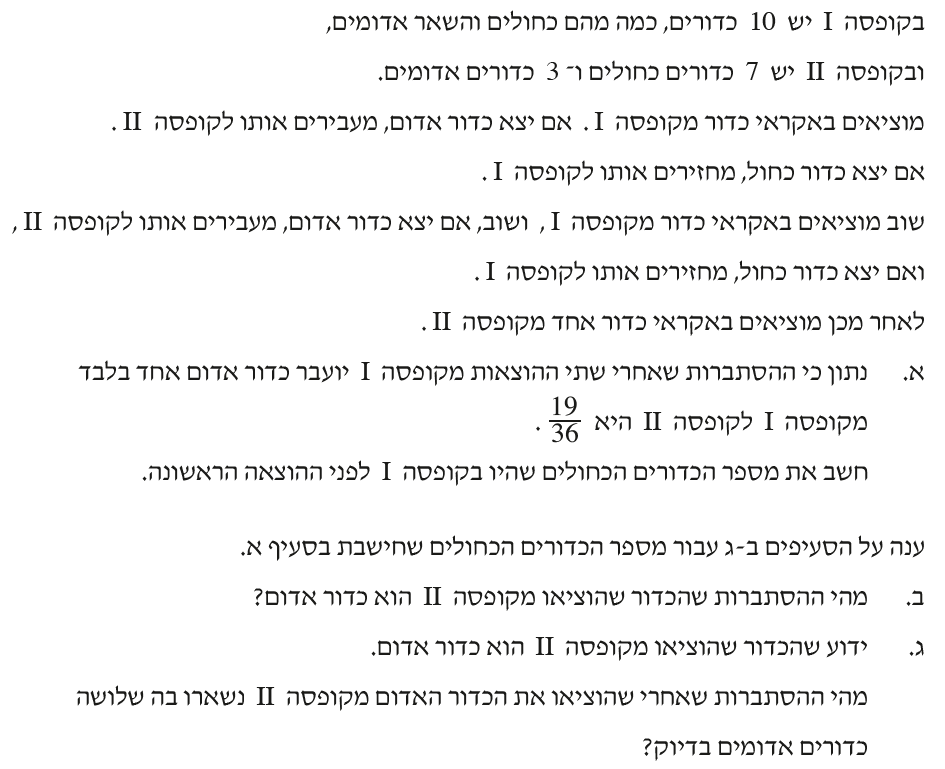
\includegraphics[width=.95\textwidth]{summer-2017b-3}
\end{center}
הניסוח "מוציאים באקראי
$\ldots$
\textbf{ולאחר מכן}
שוב מוציאים באקראי" מכוונן לשימוש בעץ. נסמן ב-%
$b$
את מספר הכדורים הכחולים בקופסה
\L{I}.
בתרשים (בעמוד הבא) בכל צומת רשום שני זוגות של מספרים: למעלה רשום מספר הכדורים האדומים ומספר הכדורים הכחולים בקופסה
\L{I}
ומתחתיו מספר הכדורים האדומים ומספר הכדורים הכחולים בקופסה
\L{II}.
על הקשתות רשום צבע הכדור שנשלף ומתחתיו ההסתברות לשלוף את הצבע. למשל, בקשת הראשונה נשלף כדור אדום וההסתברות היא מספר הכדורים האדומים 
$10-b$
חלקי מספר הכדורים בקופסה
$(10-b)+b=10$.

\begin{figure}
\begin{center}
\begin{tikzpicture}
[grow=right,
level 1/.append style={text width=2cm,level distance=5cm,sibling distance=10em},
level 2/.append style={text width=2cm,level distance=7cm,sibling distance=6em}]
\node[text width=2cm] {(10-b,b)\\(3,7)} % root
child {
  node {(10-b,b)\\(3,7)}
    child {
      node {(10-b,b)\\(3,7)}
      edge from parent node[below] {\R{כחול}}
        node[above,xshift=16mm,yshift=-2mm] {$\frac{b}{10}$}
    }
    child {
      node {(9-b,b)\ *\\(4,7)}
      edge from parent node[above] {\R{אדום}}
        node[below,xshift=16mm,yshift=2mm] {$\frac{10-b}{10}$}
    }
    edge from parent node[below] {\R{כחול}} node[above,xshift=8mm,yshift=0mm] {$\frac{b}{10}$}
}
child { 
  node {(9-b,b)\\(4,7)}
    child {
      node {(9-b,b)\ *\\(4,7)}
      edge from parent node[below] {\R{כחול}}
        node[above,xshift=16mm,yshift=-2mm] {$\frac{b}{9}$}
    }
    child {
      node {(8-b,b)\\(5,7)}
      edge from parent node[above] {\R{אדום}}
        node[below,xshift=16mm,yshift=2mm] {$\frac{9-b}{9}$}
    }
    edge from parent node[above] {\R{אדום}} 
      node[below,xshift=8mm,yshift=0mm] {$\frac{10-b}{10}$}
};
\end{tikzpicture}
\end{center}
\end{figure}

\textbf{סעיף א}

הכוכביות בתרשים מסמנות את שני המסלולים המגיעים למאורע המבוקש 
$R1$:
שנשלף כדור אדום אחד בדיוק מקופסה
\L{I}.
שתי השליפות הן זרות זו לזו ולכן ההסתברות היא סכום ההסתברות לאורך כל אחד מהמסלולים, והסתברות זו נתונה בשאלה:
\[
P(R1)=\frac{10-b}{10}\cdot\frac{b}{9} + \frac{b}{10}\cdot\frac{10-b}{10} = \frac{19}{36}\,.
\]
נפשט ונקבל משוואה ריבועית 
$b^2-10b+25=0$
שיש לה פתרון אחד
$b=5$.


\textbf{סעיף ב}

מהמידע הרשום בצד הימיני של התרשים אפשר לראות שמספר הכדורים האדומים שנמצאים בקופסה
\L{II}
הם:
$5,4,4,7$.
נסכם את ההסתברויות של המאורע
$P(R2$,
לשלוף כדור אדום מקופסה
\L{II},
לאורך כל אחד מהמסלולים כאשר קודם נציב 
$b=5$
שמצאנו לעיל:
\[
\erh{2.5}
\begin{array}{rcl}
P(R2)&=&\displaystyle\left(\frac{5}{10}\cdot\frac{4}{9}\right)\left(\frac{5}{12}\right)+
\left(\frac{5}{10}\cdot\frac{5}{9}\right)\left(\frac{4}{11}\right)+\\
&&\displaystyle\left(\frac{5}{10}\cdot\frac{5}{10}\right)\left(\frac{4}{11}\right)+
\left(\frac{5}{10}\cdot\frac{5}{10}\right)\left(\frac{3}{10}\right)
=0.3595\,.
\end{array}
\]

\textbf{סעיף ג}

הניסוח
"\textbf{ידוע ש-}"
מכוון להסתברות מותנית. המאורע החדש הוא
$P(R3)$:
נשארו שלושה כדורים אדומים בקופסה 
\L{II}:
\[
P(R3/R2)=\frac{P(R3\cap R2)}{P(R2)}\,.
\]
את
$P(R2)$
חישבנו בסעיף הקודם.

נשארו שלושה כדורים אדומים רק אם היו אברעה כדורים אדומים לפני הבחירה, מאורע 
$R4$.
ההסתברות 
$P(R4)$
למעשה נתונה
$\frac{19}{36}$,
והיא ההסתברות להגיע לאחד המצבים המסומנים בכוכבית. מכאן שההסתברות של 
$P(R3)$
היא ההסתברות להגיע לאחד מהמצבים כפול ההסתברות לשלוף כדור אדום במצב זה:
\[
P(R3)=P(R4)\cdot \textstyle\frac{4}{11}\,.
\]
ההסתברות המותנית הדרושה היא:
\[
P(R3/R2)=\frac{\frac{19}{36}\cdot\frac{4}{11}}{0.3595}=0.53385\,.
\]

%%%%%%%%%%%%%%%%%%%%%%%%%%%%%%%%%%%%%%%%%%%%%%%%%%%%%%%%%%%%%%%%%%%

\section{קיץ תשע"ז מועד א}

\begin{center}
\selectlanguage{english}
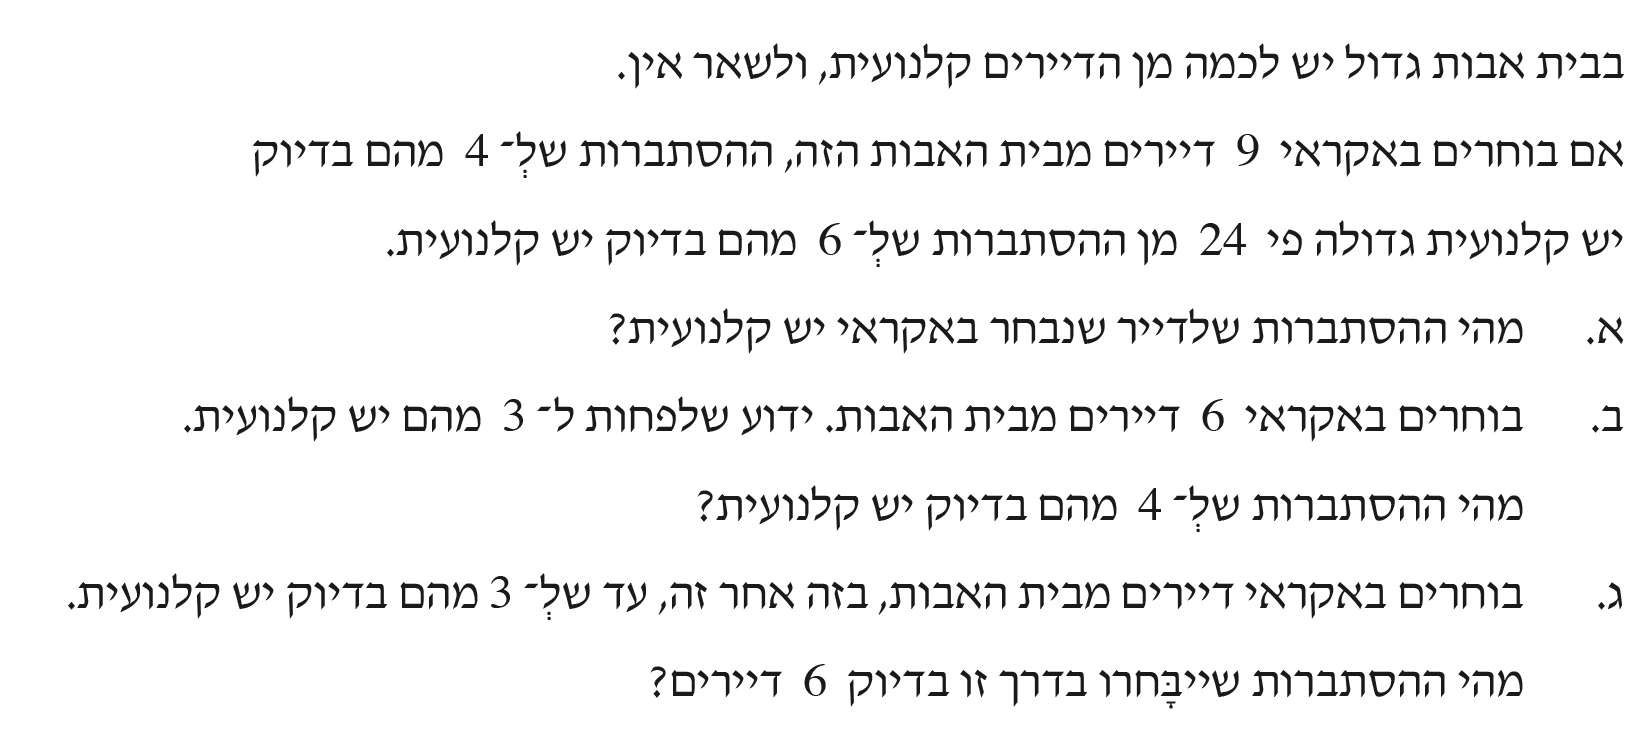
\includegraphics[width=.95\textwidth]{summer-2017a-3}
\end{center}

\textbf{סעיף א}

נסמן ב-%
$D$
את המאורע "לדייר יש קלנועית" ונסמן
$P(D)=p$.
לפי ניסוח השאלה הצלחה היא בחירת דייר עם קלנועית ונמסר מידע על "בדיוק" מספר ההצלחות, ולכן נשמתש בנוסחת ברנולי לכדי לקבל משוואה במשתנה 
$p$:
\begin{eqnarray*}
{9\choose 4} p^4 (1-p)^5&=&24 {9\choose 6} p^6 (1-p)^3\\
\frac{1}{4}(1-p)^2&=&\frac{24}{6}p^2\\
15p^2+2p-1&=&0\\
p&=&\frac{1}{5}=0.2\,,
\end{eqnarray*}
כאשר השורש 
$-\frac{1}{3}$
אינו יכול להיות פתרון כי הסתברות חייבת גדול או שווה לאפס.

\textbf{סעיף ב}

נסמן ב-%
$N$
את המאורע של "מספר הדיירים שיש להם קלנועית". הניסוח
"\textbf{ידוע ש-}"
מכוון להסתברות מותנית:
\[
P(N=4/N\ge3) = \frac{P(N=4\cap N\ge 3)}{P(N\ge 3)}\,.
\]
כאשר קבוצה אחת בחיתוך היא תת-קבוצה של השנייה, אפשר לפשט את החיתוך ולהשתמש רק בקבוצה הקטנה יותר. ברור שאם 
$N$
גדול או שווה ל-%
$3$
\textbf{וגם}
$N$
שווה ל-%
$4$
אז
$N$
שווה ל-%
$4$:
\[
P(N=4/N\ge3) =\frac{P(N=4)}{P(N\ge 3)}\,.
\]
לפי נוסחת ברנולי:
\[
P(N=4)={6\choose 4} 0.2^4 (1-0.2)^2= 0.01536\,.
\]
המונה
$P(N\ge 3)$
אפשר לחשב בשתי דרכים. בצורה ישירה:
\begin{eqnarray*}
P(N\ge 3)&=&{6\choose 3}0.2^3(1-0.2)^3+{6\choose 4}0.2^4(1-0.2)^2+\\
&&{6 \choose 5} 0.2^5(1-0.2)^1+ {6 \choose 6} 0.2^6(1-0.2)^0=0.099\,,
\end{eqnarray*}
או לפי המשלים:
\begin{eqnarray*}
P(N\ge 3)=1-P(N<3)&=&
1-0.2^0(1-0.2)^6-{6\choose 1}0.2^1(1-0.2)^5 -\\
&&{6 \choose 2} 0.2^2(1-0.2)^4=0.099\,.
\end{eqnarray*}
התשובה לשאלה היא:
\[
P(N=4/N\ge3) =\displaystyle\frac{P(N=4)}{P(N\ge 3)}=\displaystyle\frac{0.01536}{0.099}=0.15534\,.
\]
\textbf{סעיף ג}

הניסוח 
"\textbf{עד ש}"
אומר שהבחירה 
\textbf{האחרונה} 
תהיה "הצלחה" ושיהיו שתי "הצלחות" בחמשת הבחירות הקודמות. נסמן הצלחה ב-%
$+$
וכישלון ב-%
$-$
ונסדר את הדרישה בשאלה בשורה:
\[
\overbrace{\pm\;\pm\;\pm\;\pm\;\pm}^{2/5}\quad\quad \overbrace{+}^{1/1}
\]
התשובה מתקבלת מנוסחת ברנולי לבחירות הראשונות כפול ההסתברות
$p$
לבחירה האחרונה:
\[
\left[{5\choose 2}0.2^2 (1-.02)^3\right]\cdot 0.2=0.04096\,.
\]

%%%%%%%%%%%%%%%%%%%%%%%%%%%%%%%%%%%%%%%%%%%%%%%%%%%%%%%%%%%%%

\section{חורף תשע"ז}

\begin{center}
\selectlanguage{english}
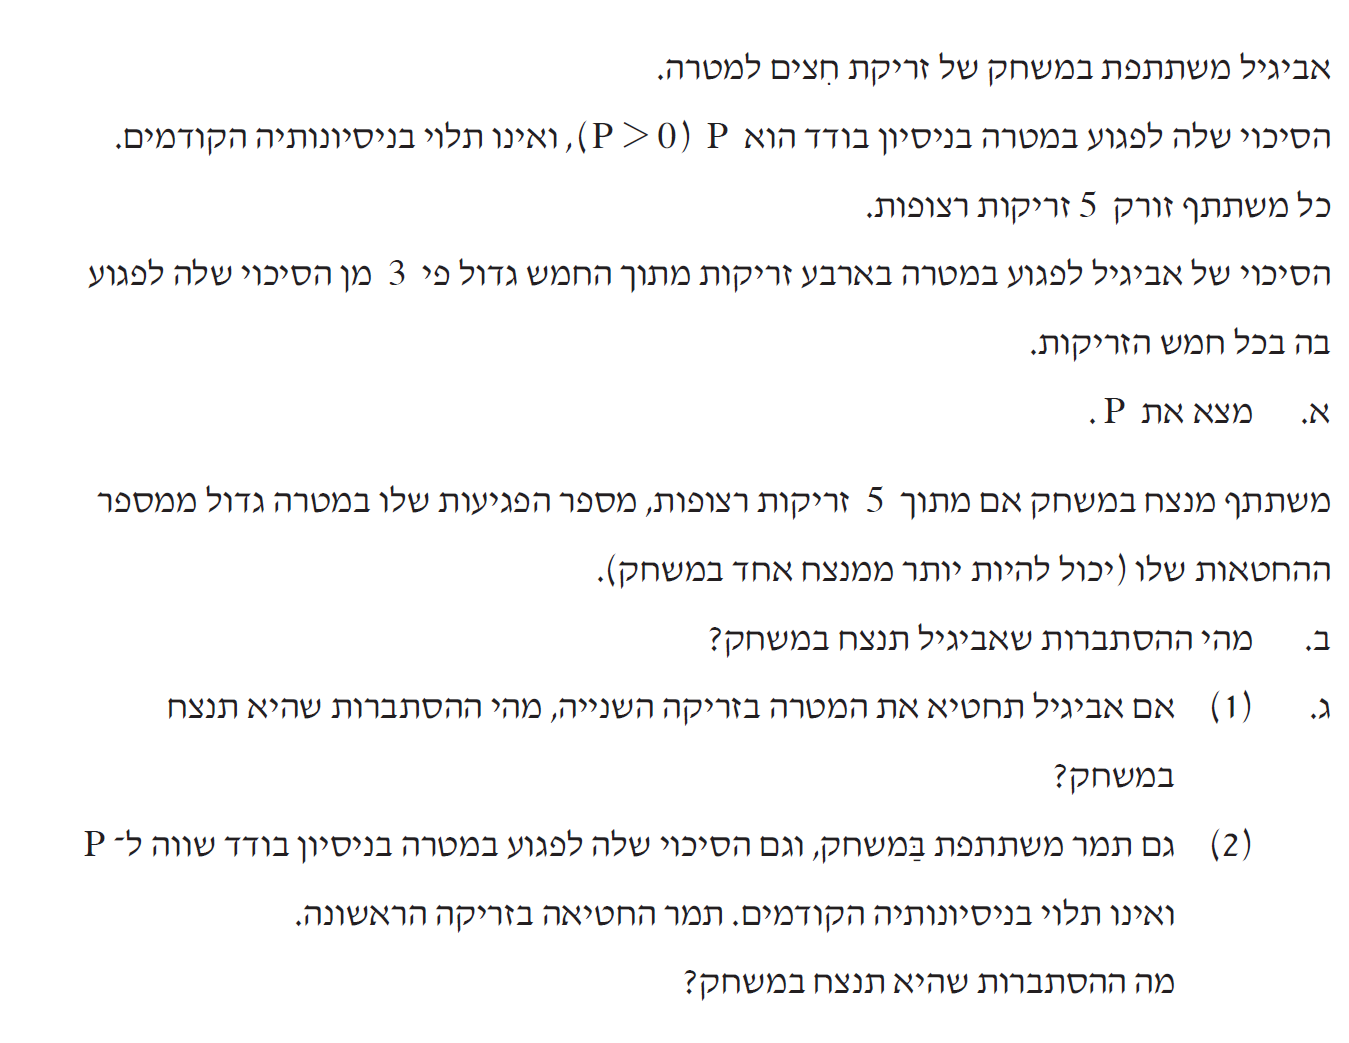
\includegraphics[width=.95\textwidth]{winter-2017-3.png}
\end{center}

\textbf{סעיף א}

נסמן ב-%
$A$
את המאורע "אביגיל פוגעת" ונסמן
$P(A)=p$.
לפי ניסוח השאלה הצלחה היא פגיעה במטרה ונמסר מידע על מספר ההצלחות, ולכן נשמתש בנוסחת ברנולי לכדי לקבל משוואה במשתנה 
$p$:
\begin{eqnarray*}
{5 \choose 4} p^4(1-p)^1 &=& 3{5\choose 5}p^5(1-p)^0\\
5(1-p) &=& 3p\\
p&=&\frac{5}{8}\,.
\end{eqnarray*}

\textbf{סעיף ב}

נסמן ב-%
$N5$
את מספר הפגיעות של אביגיל מתוך חמש זריקות. ניצחון שלה היא 
$N5\geq 3$
וההסתברות היא:
\[
P(N5\geq 3)=
{5 \choose 3}p^3(1-p)^2 + {5 \choose 4}p^4(1-p)^1 + {5 \choose 5}p^5(1-p)^0.
\]
נציב
$p=\displaystyle\frac{5}{8}$
ונקבל
$0.7248$.

\textbf{סעיף ג (1)}

לדעתי ניסוח השאלה לא ברור. אני פירשתי אותה כך: מה ההסתברות של
\textbf{המאורע}
"אביגיל מחטיאה בזריקה השנייה ופוגעת בשלוש או ארבע מהזריקות האחרות"? כותב הבחינה התכוון להסתברות מותנית: "%
\textbf{אם ידוע}
שאביגיל החטיאה בזריקה השנייה, מה ההסתברות שהיא פוגעת בשלוש או ארבע מהזריקות האחרות"?

נסמן ב-%
$T2$
את המאורע שאביגיל מחטיאה בזריקה השנייה, ונסמן ב-%
$N4$
את מספר הפגיעות שלה מתוך ארבע זריקות. ההסתברות המותנית היא:
\[
P(N4\geq 3/T2) = \frac{P(N4\geq 3\cap T2)}{P(T2)}\,.
\]
הזריקות לא תלויות אחת בשנייה ולכן:
\[
P(N4\geq 3/T2) = \frac{P(N4\geq 3)\cdot P(T2)}{P(T2)}=P(N4\geq 3)\,,
\]
ולפי נוסחת ברנולי:
\[
P(N4\geq 3/T2) =P(N4\geq 3)=
{4\choose 4}\left(\frac{5}{8}\right)^4 \left(\frac{3}{6}\right)^0 +{4\choose 3}\left(\frac{5}{8}\right)^3\left(\frac{3}{8}\right)^1 = 0.5188\,.
\]

\textbf{סעיף ג (2)}

ההסתברות של תמר לפגוע זהה להסתברות של אביגיל לפגוע ולכן ניתן להשמתמש בתוצאות שכבר חישבנו. גם לא משנה איזו זריקה החטיאה כי הזריקות בלתי תלויות, ולכן לפי סעיף ג (1) ההסתברות של תמר לנצח היא גם
$0.5188$.
